\documentclass{article}

% if you need to pass options to natbib, use, e.g.:
% \PassOptionsToPackage{numbers, compress}{natbib}
% before loading nips_2017
%
% to avoid loading the natbib package, add option 
% \usepackage[nonatbib]{nips_2017}

\usepackage[square,numbers]{natbib}
\bibliographystyle{unsrtnat}

\usepackage{nips_2017}

% to compile a camera-ready version, add the [final] option, e.g.:
% \usepackage[final]{nips_2017}

\usepackage[utf8]{inputenc} % allow utf-8 input
\usepackage[T1]{fontenc}    % use 8-bit T1 fonts
\usepackage{hyperref}       % hyperlinks
\usepackage{url}            % simple URL typesetting
\usepackage{booktabs}       % professional-quality tables
\usepackage{amsfonts}       % blackboard math symbols
\usepackage{nicefrac}       % compact symbols for 1/2, etc.
\usepackage{microtype}      % microtypography
\usepackage{graphicx}

\title{Investigation of Long Short-Term Memory Networks Implementation in cuDNN}

% The \author macro works with any number of authors. There are two
% commands used to separate the names and addresses of multiple
% authors: \And and \AND.
%
% Using \And between authors leaves it to LaTeX to determine where to
% break the lines. Using \AND forces a line break at that point. So,
% if LaTeX puts 3 of 4 authors names on the first line, and the last
% on the second line, try using \AND instead of \And before the third
% author name.

\author{
  Li Gu \\
  University of Toronto \\
  Toronto, Canada \\
  \texttt{li.gu@mail.utoronto.ca} \\
  \And
  Shuo Niu \\
  University of Toronto \\
  Toronto, Canada \\
  \texttt{shuo.niu@mail.utoronto.ca} \\
  \And
  Yang Fang \\
  University of Toronto \\
  Toronto, Canada \\
  \texttt{jake.fang@mail.utoronto.ca} \\
  %% examples of more authors
  %% \And
  %% Coauthor \\
  %% Affiliation \\
  %% Address \\
  %% \texttt{email} \\
  %% \AND
  %% Coauthor \\
  %% Affiliation \\
  %% Address \\
  %% \texttt{email} \\
  %% \And
  %% Coauthor \\
  %% Affiliation \\
  %% Address \\
  %% \texttt{email} \\
  %% \And
  %% Coauthor \\
  %% Affiliation \\
  %% Address \\
  %% \texttt{email} \\
}

\begin{document}
% \nipsfinalcopy is no longer used

\maketitle
\begin{abstract}
  In this project, we are going to implement long short-term memory networks in CUDA 
  and investigate both the computation efficiency and memory efficiency of the networks.
\end{abstract}

\section{Introduction}

% Deep neural networks (DNNs) are the state-of-art solutions to many artificial intelligence problems such as computer vision and natural language processing. At the same time powerful Graphics Processing Units(GPUs) becomes the first choice of hardware to provide acceleration for those DNNs which comes with high computation complexity and significant energy consumption.

% The two major forms of the networks are Feed-forward Neural Networks whose information is only fed forward to the next layer and Recurrent Neural Networks (RNNs) whose units in each layer form a directed graph along the sequence to form the internal memory and process sequence of inputs. Much more attention have been given to optimizing the implementation of feed-forward networks on GPUs particularly in the case of Convolutional Neural Networks (CNNs)\cite{lavin2016fast, vasilache2014fast, li2016optimizing}. As far as we know, there are a few studies on the hardware acceleration of RNNs\cite{appleyard2016optimizing}.

% One drawback of RNNs is that it cannot recognize the pattern of a sequence of inputs if there is a large gap between two related inputs. Long Short-Term Memory networks (LSTMs)\cite{hochreiter1997long} is a special kind of RNNs which was introduced to address the problem of learning long-term dependencies.



%%%%%%  Background %%%%%%%%

Recurrent Neural Networks (RNNs) are the state-of-art approaches for a large number of sequence tasks, including sequence generation\cite{eck2002first,sutskever2014sequence,gravessupervised}, machine translation \cite{cho2014learning,jean2015montreal,luong2015effective}, speech recognition \cite{graves2013speech}. LSTM \cite{hochreiter1997long}, an special RNN architecture, can avoid the issue of vanishing gradient \cite{pascanu2013difficulty} in deeper network and thus be more capable of learning long-term dependencies. A key factor in these recent success has come from the GPUs acceleration \cite{leonard2015rnn,weninger2015introducing} and Nvidia introduces cuDNN library\cite{chetlur2014cudnn} with highly-optimized implementation of RNNs\cite{appleyard2016optimizing} 

%%%%% Method in Brief 
In this project, we hope to learn GPU programming and fundamental optimization techniques in CUDA, and try to get familiar with several mainstream GPU-accelerated library in deep learning, including cuDNN and Torch. Furthemore, we hope to come up with some strategies to further maximize memory throughput for above existing libraries. The whole project will include two parts:

\begin{itemize}
  \item Firstly, we will implement a naive LSTM in CUDA and work on optimizations from cell level to layer level according to\cite{appleyard2016optimizing}, which is called cuda-LSTM.
  \item Secondly, inspired by\cite{li2016optimizing}, we will investigate the memory-efficiency among cuda-LSTM, cuda-torch\cite{PyTorch} and cuDNN by analysing the impact of data layout and the off-chip memory access

\end{itemize}

%%%%% Evaluation %%%%%%

To evaluate different optimization strategies, we will have experiments in two different levels: In CUDA level, our implemented optimization strategies will be evaluated with DeepBench\cite{DeepBench}; In application level, we will integrated our custom cuda-LSTM library into Pytorch and evaluate training and inference time in some sequence-to-sequence tasks, such as Neural Machine Translation\cite{luong2015effective}.


% Nvidia introduces the highly optimized cuDNN library\cite{chetlur2014cudnn} in 2014 and brought the support for Simple RNN, GRU, and LSTM architectures in the release of the fifth version in 2016. We would like to implement their unveiled approaches to accelerate a standard LSTM networks and search for the general portable efficient methods for accelerating different forms of RNNs architectures which would be beneficial when implementing and deploying a newly invented RNNs architecture on different GPUs. After investigation of the computation efficiency, we would turn into the memory efficiency of the network which has been significantly overlooked.

\section{Related work}

Recurrent neural networks (RNN) address the problem of recognizing patterns in sequences of data, such as text and speaking, in the way of looping the same neural network for each sequential input. However, if the input sequence is long, there could be a large gap between the current input and the previous important context. In that case, because inputs along the time steps relate to each other via multiplication, derivatives of the previous input are susceptible to become zero (called vanishing gradient) or infinity (called exploding gradient). 

Long Short Term Memory (LSTM) networks are a special kind of RNN, which is introduced to address the problem of learning long-term dependencies. LSTM cells in serial pass a hidden state, and there are four neural network layers in one LSTM cell which decides what information to be forgotten from, added in, or output from the hidden state.
\vspace{10pt}

\centerline{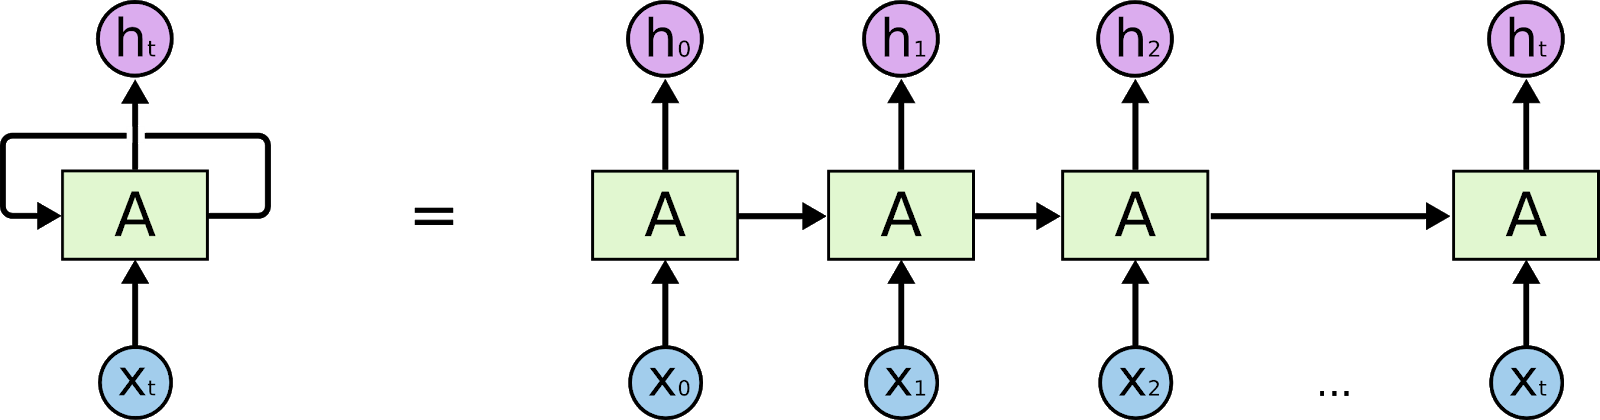
\includegraphics[width=5in]{rnn.png}}
\centerline{\textbf{Recurrent Neural Networks}}
\vspace{10pt}

\centerline{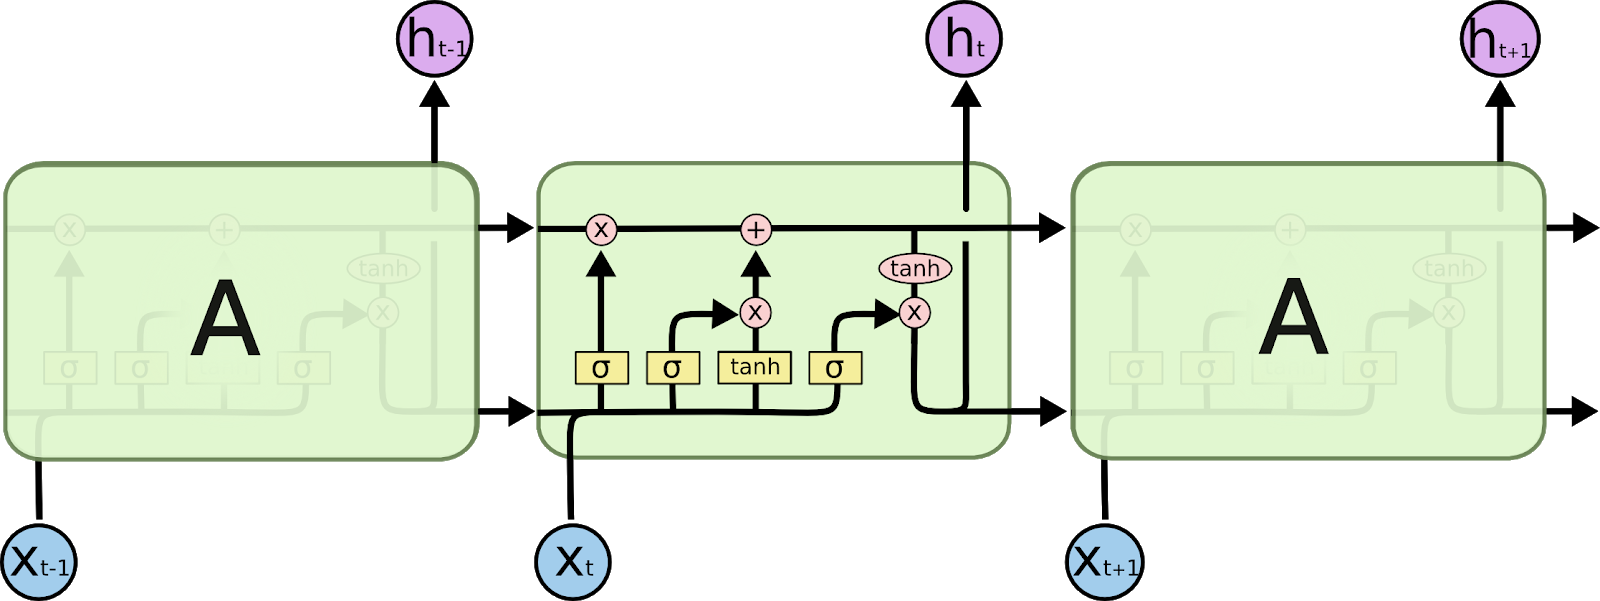
\includegraphics[width=5in]{lstm.png}}
\centerline{\textbf{The repeating module in an LSTM cell}}
\vspace{10pt}

\centerline{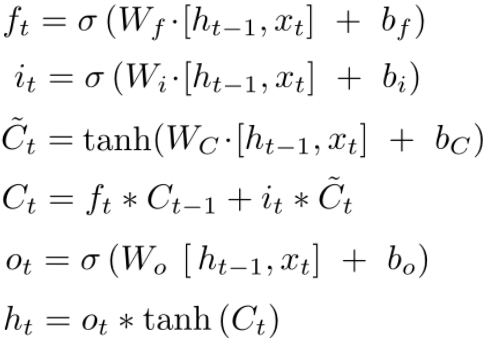
\includegraphics[width=2.1in]{lstm_formulas.png}}

Baidu DeepBench\cite{DeepBench} is one benchmark that we can use to evaluate our CUDA code on operation-level, particularly dense matrix multiplies, convolutions, and RNN. The metrics it uses are computation time and TeraFLOPS. 
PyTorch\cite{PyTorch} is a deep learning framework initially released in October 2016, which provides strong GPU acceleration for tensor computation. 
By employing DeepBench, we will benchmarking our CUDA code against underlying neural network libraries such as cuDNN, and PyTorch CUDA, in metrics time and TFLOPS.


\section{Methods}

At the beginning of our project, we will implement the optimization to LSTM which was realized in cuDNN 5\cite{appleyard2016optimizing}. The idea is that the more parallelism we give to GPUs, the higher performance they can achieve. There are three stages of optimization: on single cell, on single layer, and on multiple layers. For single cell, if a number of matrix multiplications share the same input, they can be combined into a larger matrix multiplication. Furthermore, different matrix multiplications can be computed concurrently using CUDA streams. And in addition, point-wise operations that are in separate kernels can be fused into one single kernel to reduce data transfers and cost of launching a kernel. As for single layer, the weight matrix used for this layer can be pre-transposed before doing any operation, and inputs for multiple time steps can be combined to produce a larger matrix. With regards to multiple layers, as iteration n of a given layer only depends on iteration (n-1) of the same layer and iteration n of the previous layer, it is possible to concurrently perform operations on many layers.

\medskip

\bibliography{references}

\end{document}
